\subsection{Sprint 1}

Στην ενότητα αυτή παρουσιάζονται οι τιμές των μετρικών που
χρησιμοποιήθηκαν, για κάθε κλάση/enumeration, στο τέλος του sprint 1. Υπενθυμίζεται
ότι μέχρι αυτό το σημείο η ανάπτυξη είχε ως στόχο τη υλοποίηση της
backend λειτουργικότητας του λογισμικού και δεν έχουν αναπτυχθεί ακόμα
κλάσεις γραφικής διασύνδεσης.

\subsubsection{Logical Lines Of Code (LLOC)}
\label{section:sprint1LLOC}

Στο σχήμα \ref{fig:sprint1LLOC} εμφανίζεται ο ο αριθμός των λογικών
γραμμών κώδικα ανά κλάση. Παρατηρούμε ότι η κλάση DBManager
έχει το μεγαλύτερο μέγεθος. Αυτό ήταν αναμενόμενο, λόγω του ότι η κλάση
αυτή είναι υπεύθυνη για όλες τις συναλλαγές της εφαρμογής με την τοπική βάση
δεδομένων. Αν και το μέγεθος της κλάσης δεν είναι ιδιαίτερα μεγάλο από
μόνο του, ίσως αυτό είναι ένα σημάδι ότι η κλάση DBManager θα μπορούσε να
διαχωριστεί σε μικρότερες κλάσεις.

\begin{figure}
\centering
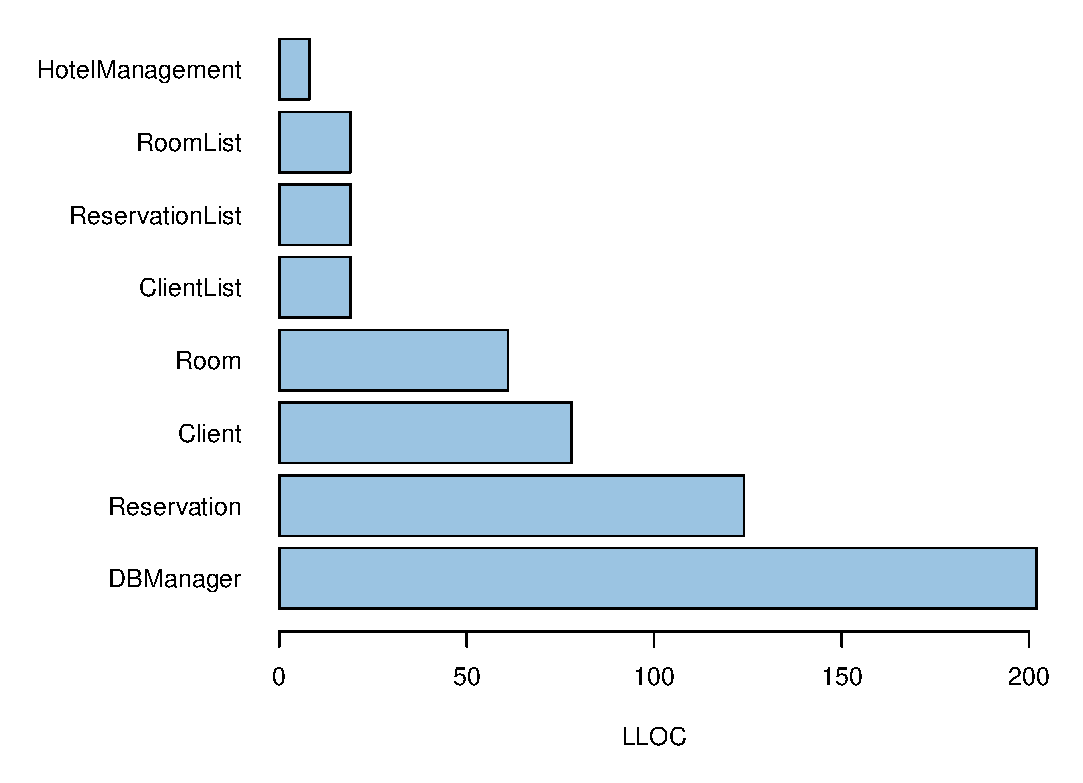
\includegraphics[width=1.0\textwidth]{Sprint1-LLOC-1.eps}
\caption{Λογικές γραμμές κώδικα ανά κλάση στο τέλος του sprint 1}
\label{fig:sprint1LLOC}
\end{figure}

Αυξημένο σχετικά μέγεθος, αλλά σε μικρότερο βαθμό παρουσιάζει επίσης η
κλάση Reservation, πράγμα επίσης αναμενόμενο, αφού τα χαρακτηριστικά
μιας κράτησης είναι εννοιολογικά περισσότερα και πιο πολύπλοκα από αυτά
των υπολοίπων κλάσεων.

\subsubsection{Clone Coverage (CC)}
\label{section:sprint1CC}

Οι τιμές της μετρικής επανάληψης κώδικα CC για τις κλάσεις του
συστήματος στο τέλος του sprint 1 εμφανίζονται στο σχήμα
\ref{fig:sprint1CC}. Οι κλάσεις που εμφανίζουν τις υψηλότερες και
ενδεχομένως ανησυχητικές τιμές είναι οι Client και Room, με πάνω από το
50\% του κώδικα να χαρακτηρίζεται ως επαναλαμβανόμενο.

\begin{figure}
\centering
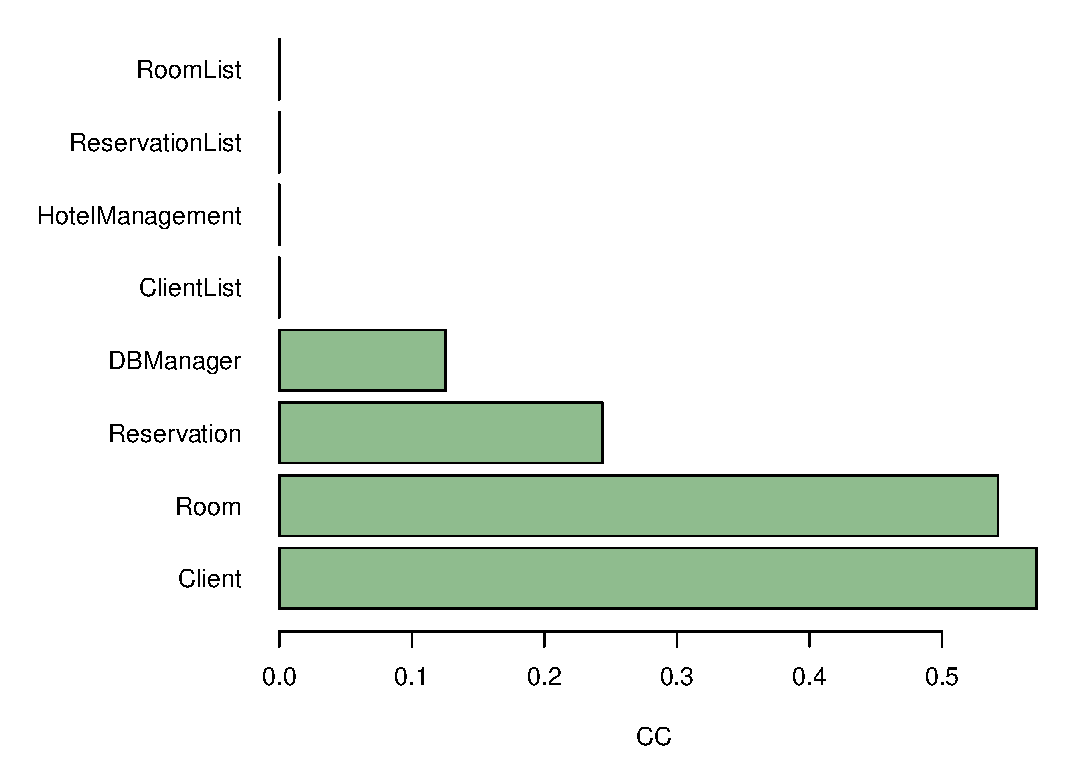
\includegraphics[width=1.0\textwidth]{Sprint1-CC-1.eps}
\caption{Τιμές της μετρικής CC ανά κλάση στο τέλος του sprint 1}
\label{fig:sprint1CC}
\end{figure}

Στο σχήμα \ref{fig:sprint1LLOC} φαίνεται πως οι κλάσεις αυτές είναι
αρκετά μικρές σε μέγεθος, συνολικά 60-70 λογικές γραμμές
κώδικα η καθεμία. Με μια ανάγνωση του κώδικα των κλάσεων αυτών είναι
εύκολο να αντιληφθεί κάποιος γιατί οι τιμές της μετρικής CC είναι τόσο
υψηλές. Σε αυτές έχει προστεθεί κώδικας ελέγχου της λειτουργικότητάς
τους στις μεθόδους main που έχουν οι κλάσεις. Ο κώδικας αυτός σε όλες
τις περιπτώσεις μοιάζει με αυτόν του πίνακα \ref{table:CCcode}.

\begin{table}
\caption{Απόσπασμα κώδικα της μεθόδου main της κλάσης Client}
\label{table:CCcode}
\begin{lstlisting}
System.out.println("Creating a new Client:");
Client c = new Client("XZ123546", "Mat", "12354313");
int retval = c.addToDB();
if (retval == 0) {
	System.out.println("OK");
} else {
	System.out.println("NOK");
}
System.out.println(c);
System.out.println("Changing the name:");
c.setName("Pat");
retval = c.updateDB();
if (retval == 0) {
	System.out.println("OK");
} else {
	System.out.println("NOK");
}
\end{lstlisting}
\end{table}

Είναι προφανές πως κάτι τέτοιο αποτελεί επανάληψη κώδικα. Αλλά οι επαναλήψεις
αυτές περικλείονται μόνο στην μέθοδο main και σε καμία άλλη. Ακόμα και
αν γινόταν πλήρης αφαίρεση της μεθόδου main από τον κώδικα, η
λειτουργικότητα της εφαρμογής δεν θα επηρεαζόταν στο παραμικρό. Οπότε
τελικά συμπεραίνεται πως το φαινομενικό πρόβλημα που υπάρχει στις
κλάσεις Client και Room σχετικά με την επανάληψη κώδικα είναι τελικά
παραπλανητικό και δεν επηρεάζει πραγματικά την ποιότητα του κώδικα. Θα
ήταν φυσικά προτιμότερο ο κώδικας ελέγχου που έχει προστεθεί πρόχειρα
στη μέθοδο main των κλάσεων να μεταφερθεί σε αντίστοιχες κλάσεις unit
testing.

Για τον ίδιο λόγο είναι σχετικά υψηλή και η τιμή της μετρικής CC για την
κλάση Reservation. Η μόνη διαφορά είναι ότι η κλάση αυτή, όπως φαίνεται
και στο σχήμα \ref{fig:sprint1LLOC} έχει συνολικά περισσότερες γραμμές
κώδικα, οπότε το ποσοστό του κώδικα που επαναλαμβάνεται στη μέθοδο main
είναι συνολικά μικρότερο.

\subsubsection{McCabe’s Cyclomatic Complexity (McCC)}
\label{section:sprint1McCC}


\begin{figure}
\centering
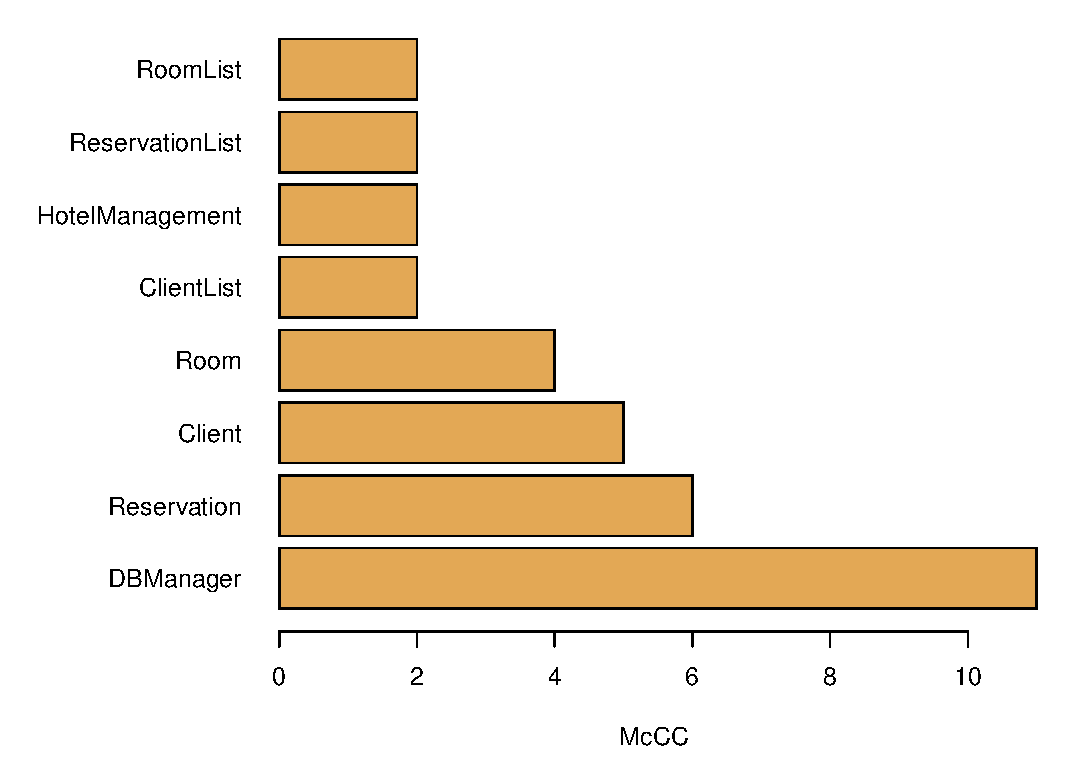
\includegraphics[width=1.0\textwidth]{Sprint1-McCC-1.eps}
\caption{Τιμές της μετρικής κυκλωματικής πολυπλοκότητας McCC ανά κλάση στο τέλος του sprint 1}
\label{fig:sprint1McCC}
\end{figure}

\subsubsection{Lack of Cohesion in Methods 5 (LCOM5)}
\label{section:sprint1LCOM5}

\begin{figure}
\centering
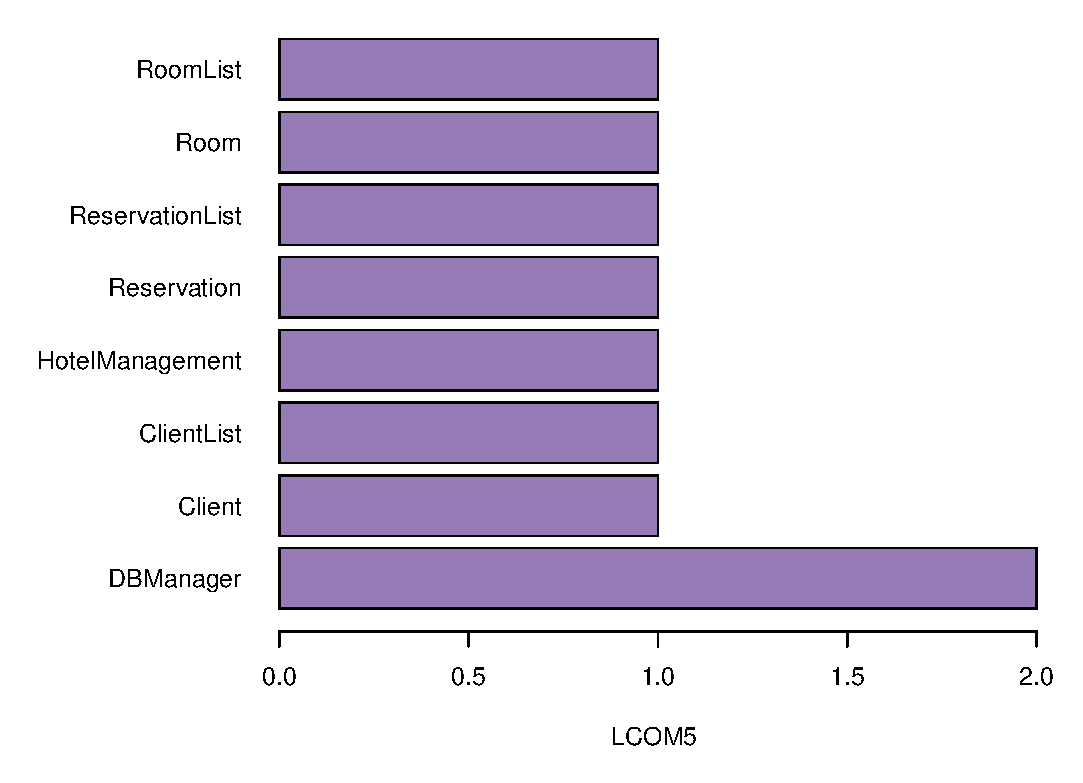
\includegraphics[width=1.0\textwidth]{Sprint1-LCOM5-1.eps}
\caption{Τιμές της μετρικής έλλειψης συνεκτικότητας LCOM5 ανά κλάση στο τέλος του sprint 1}
\label{fig:sprint1LCOM5}
\end{figure}

\subsubsection{Coupling Between Object classes (CBO)}
\label{section:sprint1CBO}

\begin{figure}
\centering
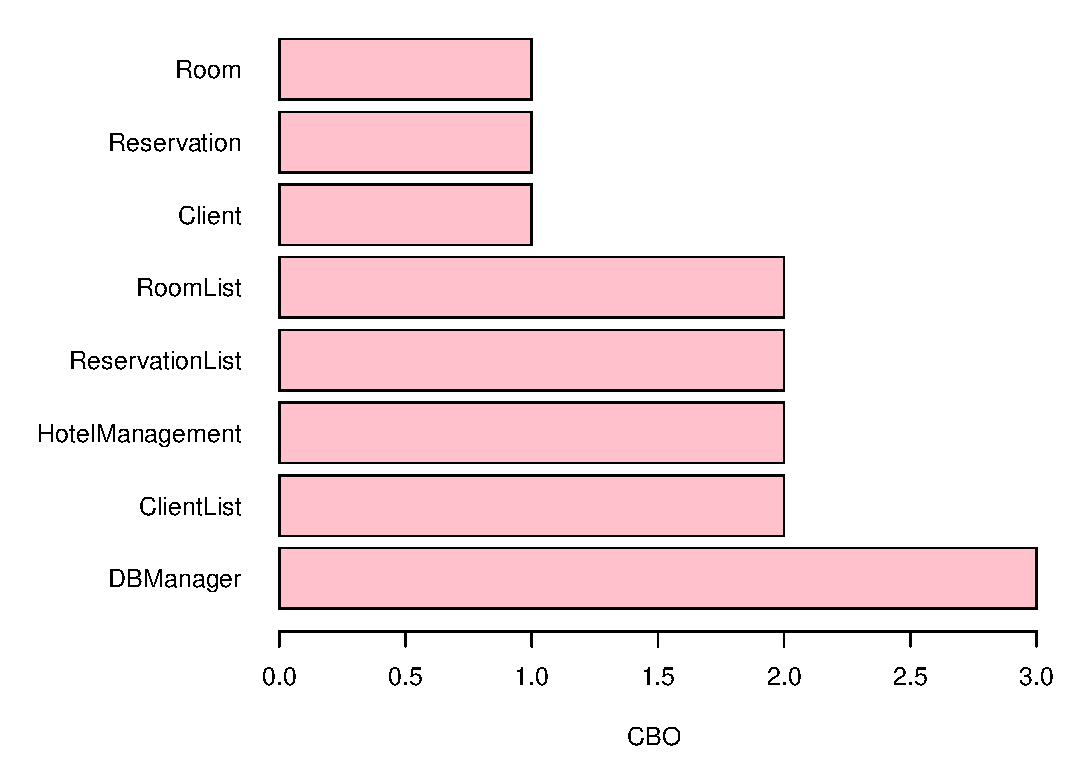
\includegraphics[width=1.0\textwidth]{Sprint1-CBO-1.eps}
\caption{Τιμές της μετρικής σύζευξης CBO ανά κλάση στο τέλος του sprint 1}
\label{fig:sprint1CBO}
\end{figure}
